%kate: default-dictionary en;

\documentclass[eprint]{actapoly}

\usepackage{algorithm}
\usepackage{algpseudocode}
\usepackage{amssymb}
\usepackage{tikz}

%\usepackage{draftwatermark}
%\SetWatermarkText{DRAFT}
%\SetWatermarkScale{1}
%\SetWatermarkLightness{0.9}

\begin{document}

%\title[Example of an Article with a Long Title]
%{Example of an Article with a Long Title, the Title Should Be Capitalised 
%Properly in the Code Long Long}
\title[Trajectory Generation Approach]
{Multi Robot Optimal Trajectory Generation}

\author[J. M. Mendes Filho]{Jos\'{e} Magno Mendes Filho}{my,their}
\correspondingauthor[E. Lucet]{Eric Lucet}{my}{eric.lucet@cea.fr}

\institution{my}{CEA, LIST, Interactive Robotics Laboratory, Gif-sur-Yvette, 
F-91191, France}
\institution{their}{ENSTA Paristech, Unit\'{e} d'Informatique et d'Ing\'{e}nierie 
des Syst\`{e}mes, 828 bd des Marechaux, 91762, France}
%\institution{their}{ENSTA Paristech, Unit\'{e} informatique et Ingénierie des 
%Système, 828 boulevard des Marechaux, F-91762, France}
%\institution{their}{CEA, LIST, Interactive Robotics Laboratory, 
%Gif-sur-Yvette, F-91191, France}

\begin{abstract}
 Abstract.
\end{abstract}

\keywords{multi robot path planning, mobile robot}

\maketitle




\section{Introduction}




%General Context

The %command and
control of mobile robots is a long-standing subject of research 
in the iterative robotics domain. As many modern companies started to adopt 
mobile robot systems such as teams of autonomous forklift trucks~\cite{Gizmag} 
to improve their commercial performance, this subject becomes increasingly 
important and complex. Especially when those robots are executing theirs tasks 
in human-occupied environment.

%Problem

One basic requirement for such robotic systems is the capacity of generating a 
trajectory that connects two arbitrary configurations. For that, different 
constraints must be taken into account to ideally find an appropriated 
trajectory, in particular:

\begin{itemize}

 \item kinematic and dynamic constraints;

 \item geometric constraints;

 \item constraints associated with uncertainties about the current state of 
world and the outcome of actions.

\end{itemize}

The first constraints derive directly from the mobile robot architecture 
implying in nonholonomic constraints for many types of mobile robots. Geometric 
constraints result from the impossibility of the robots to assume some specific 
configurations due to the presence of obstacles or environment bounds. In turn, 
uncertainty constraints come from the impossibility of the robots to have an 
absolute and complete perception of the world (including theirs own states) as 
well as the outcome of non-stochastic events.

 

We are particularly interest in solving the problem of dynamic planning a 
trajectory for a team of nonholonomic mobile robots in an partially known 
environment occupied by static obstacles being near optimal with respect to the 
execution time (time spent from going from initial to final configurations).

 

%State of Art

In recent years, a great amount of work towards collision-free trajectory 
planning has been proposed.

 

Some work has been done towards analytic methods for solving the problem for 
certain classes of systems (~\cite{}). However~\cite{schwartz1988survey} shows 
that analytic methods  are inapplicable for nonholonomic systems in presence of 
obstacles.

 

Cell decomposition methods as presented in~\cite{latombe2012robot} have the 
downside of requiring a structured configuration space and an \textit{a priori} 
model of its connectivity. Besides, the cell decomposition reduces the space 
of admissible solutions. TODO verify/understand.

 

Initially proposed in~\cite{Khatib1986}, the vector field obstacle avoidance 
method was improve along time for treating problems such as oscillation of the 
solution for narrow passages. This method does not present a near optimal 
generated trajectory.

 

Elastic band approach initially proposed by~\cite{Quinlan1994} and extend to 
mobile manipulators in~\cite{Brock et Khatib, 1998} uses approximations of the 
trajectory shape (combinations of arcs and straight lines) limiting the space 
of solutions and make this method inappropriate for really constrained 
environments.

 

The dynamic window approach~\cite{fox1997dynamic} can handle trajectory 
planning for robots at elevated speeds and in presence of obstacles but is not 
flexible enough to be extended to a multi robot system.

 

%What do we propose

In this paper, we focus on the development of a motion planning algorithm. 
This algorithm finds collision-free trajectories for a multi robot system in 
presence of static obstacles which are perceived by the robots as they evolve 
in the environment. The dynamic trajectories found are near optimal with 
respect to the total time spend going from the initial configuration to the 
final one. Besides, this algorithm uses a decentralized approach making the 
system more robust to communication outages and individual robot failure than 
compared to a centralized approach. Identified drawbacks are the dependence on 
several parameters for achieving real-time performance and good solution 
optimality, and not being able to handle dynamic obstacles as it is.

 

This algorithm is based mainly on the work done in~\cite{Defoort2007a} but we 
made changes in particular to respect a precise final configuration for the 
multi robot system and about how to set parameters for solving the nonlinear 
programming problem (NLP).

 

%Plan

This paper is structured as follows: The second section presents a trajectory 
planning algorithm that solves the problem of one robot going from an initial 
configuration to a final one in the presence of static obstacles. The third 
section extends the method presented in the second section so a collision-free 
trajectory that maintains the communication link between the robots in the 
team can be computed. The forth section is dedicated to the results found by 
this method and the analysis of the computation time and solution quality and 
how they are impacted by the algorithm parameters. The fifth section presents 
the comparison of this approach to another one presented in~\cite{}. Finally, in 
section six we present our conclusions and perspectives.

\section{Problem Formulation}

%We consider the following assumptions for the simulation of our approach:
\subsection{Assumptions}
In the development of this approach the following assumptions were made:

\begin{enumerate}

    \item The team of robots consists of a set $\mathcal{R}$ of $B$
    nonholonomic mobile robots;
    
    \item A robot (denoted $R_b,\ R_b \in \mathcal{R},\ b \in \{0,\dots,B-1\}$) is 
    geometrically represented by a circle of radius $\rho_b$;
        
    \item All obstacles in the environment are considered static. They can be
    represented by a set $\mathcal{O}$ of $M$ static obstacles;
    
    \item An obstacle (denoted $O_m,\ $\mbox{$O_m \in \mathcal{O}$}$,\ $
    \mbox{$m \in \{0,\ \dots, M-1\}$}) is geometrically represented either as
    circle or as a convex polygon;
    
    \item For a given instant $t_k \in [t_{init},\ t_{final}]$, any obstacle
    $O_m$ closer to the geometric center of the robot $R_b$ to the having its
    geometric center within the detection radius $d_{b,sen}$ from
    the geometric center of the robot $R_b$ is considered detected by the robot
    $R_b$. Thus, this obstacle is part of the set $\mathcal{D}$
    ($\mathcal{D} \subset \mathcal{O}$) of detected obstacles;
    
    \item A robot has precise knowledge of the position and geometric representation of
    a detected obstacle;
    
    \item A robot can access 
    information about any robot in the team using 
    a wireless communication link.
    
    \item Latency, communication outages and other problems associated
    to the communication between robots in the team are neglected;
        
    \item Dynamics was neglected.
    
    \item The input of a mobile robot $R_b$ is limited.
    
%    \item The motion planner in a robot $R_b$ (with $n \in {0,\dots,B-1}$) has
%    access to the following information:
%    \begin{enumerate}
%        \item current and past configuration of the robot $R_b$;
%        \item $R_b$'s goal configuration;
%        \item $R_b$'s input limits;
%        \item The map function to pass from flat space to state and input space and
%        its inverse;
%        \item  
%    \end{enumerate}

%     as well as the its robot's goal configuration, the input limits,
%    its kinematic
%    model and bijective mapping function for passing from the flat space to the
%    actual state and input spaces;
%    
%    \item Each robot have sensors that can detect the surrounding region within a
%    radius $\rho_d$. Any object having its geometric center within this region is
%    considered detect by the robot;

\end{enumerate}

\subsection{Constraints and cost functions}

After loosely defining what is the motion planning problem in
Section~\ref{sec:intro} and presenting the assumptions in the previous Subsection
we can identify and define what are the constraints and the cost function for the
multi robot navigation.

\begin{enumerate}

    \item The system kinetic model must hold for a computed solution to the
    motion planning problem problem:
    \begin{equation}
        \dot{q}_b = f(q_b,u_b)
    \end{equation}
	with $q_b\,:\,\mathbb{R}^{+}\rightarrow \mathbb{R}^n$ the robot's configuration
	vector,
	$u_b\,:\,\mathbb{R}^{+}\rightarrow \mathbb{R}^p$ the robot's input vector and
	\mbox{$f\,:\,\mathbb{R}^{n}\times \mathbb{R}^{p}\rightarrow \mathbb{R}^n$} the
	vector field.
    
    \item The practical limitations of the input can be taken into account by the
    following constraint:
    \begin{equation}
        |u_{b,i}| \leq u_{b,i,max}\quad \forall i \in [1, p]
    \end{equation}
    
    \item The cost for the multi robot system is defined as:
    \begin{equation}
        L(q,u) = \sum_{b=0}^{B-1}L_b(q_b, u_b, q_{b,final})
    \end{equation}
    where $L_b(q_b, u_b, q_{b,final})$ is the integrated cost for one robot
    stabilisation (see~\cite{Deffort2009});
    
    
    \item 
    %TODO define the functions "distance" robot-to-obstacle:
    To ensure collision avoidance with obstacles the euclidean 
    distance between
    a robot and an obstacle (denoted $\mathrm{d}(R_b, O_m)\ |\ O_m
    \in \mathcal{O}_b, R_b \in \mathcal{B} $) has to satisfy:
    \begin{equation}
    	\mathrm{d}(R_b, O_m) > 0
    \end{equation}
    For the circle representation of an obstacle the distance
    $\mathrm{d}(R_b, O_m)$ is defined as:
    \begin{equation*}
        \sqrt{(x_{b} - x_{O_m})^2 + (y_{b} - y_{\mathrm{O}_m})^2}  - \rho_b - r_{O_m}
    \end{equation*}
    with $r_{O_m}$ being the obstacle radius.
    
    For the polygon representation, the distance was calculated using three different
    definitions according to the Voronoi region~\cite{ericson2004real}
    within which
    $R_b$ is located. Figure~\ref{fig:convexpolygon} shows an example of the thee kind
    of regions for a quadrilateral $ABCD$ representation. The regions are defined by
    the lines containing the sides ($s$ lines) and by the lines passing
    through the vertices that are orthogonal to the sides ($r$ lines).    
    
	The region in which the robot $R_b$ is located
	can be computed by evaluating the line
 	equations 
 	$s_{AB}$, $s_{BC}$, $s_{CD}$, $s_{DA}$, $r_{AB}$, $r_{AD}$, $r_{BA}$, $r_{BA}$,
 	$r_{BC}$, $r_{BA}$, $r_{BC}$, $r_{CB}$, $r_{CD}$, $r_{DC}$ and $r_{DA}$ for 
 	the position associated with the configuration $q_b$.
 	
%    The region which the position associated with a given configuration $q_b$
%    is in can be computed as follows.
    
    For the example in the Figure~\ref{fig:convexpolygon} the distance
    robot-to-quadrilateral could be found as follows:
    \begin{enumerate}
    
	   	\item If robot in region $1$:
   	   	\begin{equation*}
    	    \sqrt{(x_{b} - x_{A})^2 + (y_{b} - y_{A})^2} - \rho_b
	    \end{equation*}
	    which is simply the distance of the robot to the vertex $A$.
	    
	    \item If robot in region $2$:
%	    
		\begin{equation*}
			\mathrm{d}(s_{DA}, (x_{b}, y_{b})) - \rho_b
		\end{equation*}
		where
   	   	\begin{equation*}
    	    \mathrm{d}(s_{DA}, (x_{b}, y_{b})) =\\ \frac{|a_{s_{DA}}x_{b} + b_{s_{DA}}y_{b}
    	    + c_{s_{DA}}|}{\sqrt{a_{s_{DA}}^2 + b_{s_{DA}}^2}}
	    \end{equation*}
	    The distance $\mathrm{d}(s_{DA}, (x_{b}, y_{b}))$ represents from the robot to the side $DA$.
	    
	    \item If robot in region $3$:
   	   	\begin{equation*}
    	    -\min\left(\mathrm{d}(s_{AB}, (x_{b}, y_{b})), \cdots, \mathrm{d}(s_{DA}, (x_{b}, y_{b}))\right) - \rho_b
	    \end{equation*}
	    which represents the amount of penetration of the robot in the obstacle.
	    
    \end{enumerate}
    \begin{figure}[!h]
	\centering
	{
    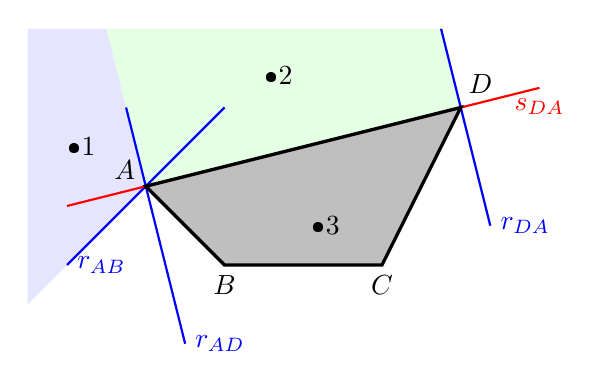
\begin{tikzpicture}
	[cube/.style={very thick,black}, 			
	grid/.style={very thin,gray},
	cube_hidden/.style={very thick,dashed},
	polygon/.style={very thick, black},
	axis/.style={-,blue,thick},
	point/.style={very thick,black},
	afill/.style = {fill=blue!20,fill opacity=0.5},
	bfill/.style = {fill=green!20,fill opacity=0.5}]
	\fill[afill] (0,1,0) -- (-0.5,3,0) -- (-1.5,3,0) -- (-1.5,-.5,0) --cycle;
	\fill[bfill] (0,1,0) -- (4,2,0) -- (3.75,3.,0) -- (-0.5,3,0) --cycle;
	\draw[axis] (-.25,2.,0) -- (.5,-1.,0) node[anchor=west,color=blue]{$r_{AD}$}; % y = 1. - 4.x
	\draw[axis] (1.,2.,0) -- (-1.,0.,0) node[anchor=west,color=blue]{$r_{AB}$};%y = x+1
	\draw[axis] (3.75,3.,0) -- (4.375,0.5,0) node[anchor=west,color=blue]{$r_{DA}$}; %y = 18.-4. x
	%\draw[axis,red] (0.,0.,0) -- (4.25,0.,0) node[anchor=west,color=red]{$s_1$};
	%\draw[axis,red] (2.75,-.5,0) -- (4.5,3.,0) node[anchor=west,color=red]{$s_2$};
	\draw[axis,red] (-1.,.75,0) -- (5.,2.25,0) node[anchor=north,color=red]{$s_{DA}$};
	%\draw[axis,red] (-0.5,1.5,0) -- (1.5,-.5,0) node[anchor=east,color=red]{$s_4$};
	
	\draw[point] (2.0,2.4,0) node[anchor=east]{\textbullet $2$};
	\draw[point] (-0.5,1.5,0) node[anchor=east]{\textbullet $1$};
	%\draw[axis] (2.0,1.0,0) -- (-0.5,-1.5,0) node[anchor=west,color=blue]{$r_{1,0}$};
	
	\draw[polygon,fill=gray!50] (0,1,0)  -- (1,0,0) node[below] {$B$} -- (3,0,0) node[below] {$C$} -- (4,2,0) -- cycle;
	\draw[point] (2.6,0.5,0) node[anchor=east]{\textbullet $3$};
%node[above] {$A$} node[above] {$D$}
	\node[text width=0cm] at (-0.4,1.2,0) {$A$};
	\node[text width=0cm] at (4.1,2.3,0) {$D$};
	\end{tikzpicture}}
	\caption{Voronoi regions used for case differentiation. \label{fig:convexpolygon}}
	\end{figure}

    \item 
    In order to prevent inter-robot collision the following constraint must be respected:
    $\forall\ (R_b, R_c) \in \mathcal{R} \times \mathcal{R}, b\neq c$,
    %o a robot $R_b$ avoid collision with other robots the following
    %relation must be satisfied. 
%    In order to avoid inter-robot collision the following constraint
%    must be respect by the robots $R_b$ and $R_b$:
    \begin{equation}
	    \mathrm{d}(R_b,R_c) - \rho_b -\rho_c > 0
    \end{equation}
    where $\mathrm{d}(R_b,R_c) = \sqrt{(x_{b} - x_{c})^2 + (y_{b} - y_{c})^2}$.
    This constraint justifies the need for a communication link between the robots.
    
    \item In order to keep the communication between robots $(R_b, R_c)$ the
    following equation must be respected: 
    %In addition, for a given pair of robots $R_b R_c$ that must keep
    %a communication link between them the following equation 
    \begin{equation}
    	\mathrm{d}(R_b,R_c)  - \min(d_{b,com}, d_{c,com}) < 0
    \end{equation}
    with $d_{b,com}, d_{c,com}$ being the communication link reach of the robots.
\end{enumerate}

\section{Distributed motion planning}

\subsection{Receding horizon approach}

%Defoort give in \cite{Defoort2007a} an example showing how a unicycle model 
%can be written using the flatness property.
%The basis algorithm for planning for a mono robot is based on the optimization 
%problem shown in equations~\ref{eq:} and~\ref{eq:}.
%TODO present method or make reference to Defoort introducing $T_c$, $T_p$ etc.

As said before trying to find the solution from the initial configuration
until the goal is not feasible. Thus, the planning has to be computed on-line
as the multi robot system evolves in the environment.
One way to do so is to use a receding horizon approach~\ref{}.

All robots in the team use the same constant planning horizon $T_p$ and update
horizon $T_c$. $T_p$ is the time horizon for which a solution will be computed,
$T_c$ is the time horizon during which the plan will be followed (usually this
is the time needed to solve the planning problem for $T_p$).

For each receding horizon planning problem the following is done:
\paragraph{Step 1.} Compute intended trajectory by ignoring coupling constraints
\paragraph{Step 2.} Robots involved in a conflict update their trajectories
by solving another optimal problem that take into account coupling constraints
using the other robots' intended trajectories computed in the first step.

%One way of modelling the motion planning problem would be to write a NPL
%that accounts for all robots 
%
%Modeling the 
%At this point a nonlinear programming problem can be written as in the
%equations~\ref{eq:objfunc} to~\ref{eq:lastconst} for finding the
%B-spline parameters that can minimize the mission time respecting some constraints.
%
%The equations~\ref{eq:qi} and~\ref{eq:qf} express the we see a first group of constraints that are expressed
%as equations
%a NLP 
%
%

\mbox{}

However, two aspects of the implementation of this algorithm are neglected 
in~\cite{Defoort2007a}: the initial values for
the control points and the procedure for reaching the goal state.

%\begin{align}
%\underset{(C_{(0,\tau_k)},\dotsc,C_{(d+n_{knot}-2,\tau_k)})}{\mathrm{min}} J_{\tau_k} =
%\nonumber\\
%\|\varphi_1(z(\tau_k+T_p,\tau_k),\dotsc,z^{(l-1)}(\tau_k+T_p,\tau_k))-q_{final}\|^2
%\end{align}
%
%under the following constraints $\forall t \in [\tau_k, \tau_k+T_p]$:
%\begin{equation}%\label{eq:sysr4}
%\left\lbrace\begin{array}{lcl}
%	\varphi_1(z(\tau_{k},\tau_{k}),\dotsc,z^{(l-1)}(\tau_k,\tau_k)) & = &  q_{ref}(\tau_k,\tau_{k-1})\\
%    \varphi_2(z(\tau_{k},\tau_{k}),\dotsc,z^{(l)}(\tau_k,\tau_k)) & = & u_{ref}(\tau_k,\tau_{k-1})\\
%    \varphi_2(z(t,\tau_k),\dotsc,z^{(l)}(t,\tau_k)) &\in& \mathcal{U}\\
%    d_{O_m}(t,\tau_k) &\geq& \rho + r_m,\quad \forall O_m \in \mathcal{O}(\tau_k)
%\end{array}\right.
%\end{equation}
%

%The following pseudo code explains the planning process. Procedures PlanSec
%and PlanLastSec formulate the NLP and
%call the an optimization method that can handles equations and inequations 
%constraints.


%A flat system has the important property that the states and the inputs
%can be written in terms of the outputs $z$ and their derivatives. Thus, the 
%behavior
%of the system is determined by the flat outputs. Note that the map w is 
%bijective(simple unicycle and simple car models for instance)
%have what is called flatness property~\ref{TODO}. 

%This property means that TODO.

%TODO system flatness

%TODO put image of the rejected trajectory??

%\begin{algorithm}[h]
%\begin{algorithmic}
%%\While{$d_{rem} \geq d_{min} + T_c \times v_{max}$}
%%\State \Call{{\scshape plan_sec}}{a}
%%\EndWhile
%%\Stae \Call{{\scshape rescale_pbl}}{a}
%%\State \Call{{\scshape plan_last_sec}}{a}
%\Function {{\scshape hpn}}{$currentState, goal , operators, absLevel , world$}
%	\If {holds(goal , currentState)}
%		\State \Return {\scshape True}
%	\Else
%    	\State $p \gets ${\scshape plan}$(currentState, goal , operators, 
%absLevel)$
%		\For {$(o_i , g_i ) \in p$}
%			\If {{\scshape prim}$(o_i)$}
%				\State $currentState \gets world.${\scshape 
%execute}$(o_i)$
%			\Else
%            	\State \Call{{\scshape hpn}}{$currentState, g_i , operators, 
%${\scshape nextLevel}$(absLevel, o_i), world$}
%    		\EndIf
%        \EndFor
%    \EndIf
%\EndFunction
%\end{algorithmic}
%\end{algorithm}

%\subsection{Flatness property}
%
%As explained in~\cite{Defoort2007a} all mobile robots consisting of a solid
%block in motion can be modelled as a flat system. 
%This means that a change of variables is possible in a way that states and
%inputs of the kinetic model of the mobile robot can be written in terms
%of the new variable, called flat output ($z$), and its $l$th first derivatives.
%Thus, the behaviour of the system can be completely determined by the flat
%output.
%
%TODO put image of flat bijective application.
%
%Searching for a solution to our problem in the flat space rather than in
%the actual configuration space of the system present advantages.
%It prevents the need for integrating the differential equations
%of system and reduces the dimension of the problem of finding an optimal
%admissible solution to the problem.
%After finding (optimal) trajectories in the flat space it is possible
%to retrieve back the original state and input trajectories as shown in
%Figure~\ref{fig:flatness}.
%
%\subsection{Parametrization of the flat output}
%
%Another important aspect of this approach is the parametrization of 
%the flat output trajectory. As done done in~\cite{milam2003} the use
%of B-spline functions present interesting properties:
%
%
%\begin{itemize}
%
%
% \item It is possible to specify a level of continuity $C^k$ when using B-splines without
% additional constraints.
% 
% \item B-spline presents a local support, i.e., changes in parameters values have a local
% impact on the resulting curve.
% 
% 
%\end{itemize}
%
%The first property is very well suited for parametrizing the flat output since
%its $l$th first derivatives will be needed when computing the system actual state
%and input trajectories. The second property is important when searching for an
%admissible solution in the flat space; such parametrization is more efficient
%and well-conditioned than, for instance, a polynomial parametrization.
%
%\subsection{NLP initialization and objective function}
%
%
%%\subsection{Solving NLP}
%The initialization of the solution paths used for each NLP solving is important 
%for two reasons:
%\begin{itemize}
%
% \item
%A good initialization allows the
%optimization solver to find a better solution for a given timespan.
% \item
%When using a local optimization method the initialization
%can drag the final solution to one or other local minima.
%\end{itemize}
%
%The simplest of initializations was performed in ours studies. Linear spacing 
%from current flat output value to the estimate final flat output.
%The estimate final output is simply the flat output computed from the estimate 
%final states and inputs. The estimate final states and inputs
%are computed assuming a displacement from the current position of the maximum 
%linear speed
%of the robot times the planning horizon, and assuming that the direction of the 
%movement is equal to (final position - current pos) vector.
%
%TODO talk about the too close obstacles problem and the dumb solution.

\subsection{Motion planning termination}


As the robots evolve theirs states approximate to the goal states.
%That is the  since the distance between current and final state is what is to 
%be minimized.
But simply stopping the motion planner as the robots are in the neighbourhood of
their final configuration is not a satisfying approach.

We propose 
At some point the constraints associated to the final state shall be integrated 
into the optimal problem and the timespan for performing this last
step shall not be fixed and must be one of the values calculated.
%The fixed planning horizon has to be made variable in order to get to the 
final state.

The criterion used to pass from the NLP used during for the initial and 
intermediates steps to the last step NLP 
is define below in the equation~\ref{eq:stopcond}:

\begin{align}
  d_{rem} \geq d_{min} + T_c \cdot v_{max}
\end{align}

This way we insure that the last planning section will be done for at least a 
$d_{min}$ distance from the robot's final position.
This minimal distance is assumed to be sufficient for the robot to reach the 
final state.

After stopping the sliding window algorithm we calculate new parameters for the 
solution representation and computation taking into
account the estimate remaining distance.

The following pseudo code summarizes the algorithm: 

\begin{algorithm}
    \caption{Sliding window planning algorithm\label{cod:algo}}
    \label{swpa}
    \begin{algorithmic}[1] % The number tells where the line numbering should start
        \Procedure{Plan}{} %\Comment{The g.c.d. of a and b}
	    \State $knots \gets $\Call{GenKnots}{$t_p,d_{spl},n_{knots}$}
	    \State $time \gets $\Call{LineSpacing}{$0,t_p,n_{s}$}
	    %\State $z_{latest} \gets $\Call{$\varphi_0$}{$q_{initial}$}
	    \State $q_{latest} \gets q_{initial}$
	    %\State $ctrlpts \gets $\Call {InitCtrlPts}{$q_{initial},q_{final},T_p,u_{max}$}
	    %\State \Call{Init}{}
	    \State $d_{rem} \gets |${\scshape Pos}$(q_{final}) - ${\scshape Pos}$(q_{latest})|$
	    \While{$d_{rem} \geq d_{min} + T_c \cdot v_{max}$}	
		\State $q_{latest} \gets $\Call{PlanSec}{}
		\State $d_{rem} \gets |${\scshape Pos}$(q_{final}) - ${\scshape Pos}$(q_{latest})|$
		
	    \EndWhile\label{planningwhile}
	    %\State \Call{RescalePbl}{}
%	    \State $s \gets $\Call {Min}{$\tfrac{d_{rem}}{v_{max}\cdot t_p}, 1.0$}
%	    \State $n_{knots} \gets $\Call{Max}{\Call{Round}{$s\cdot n_{knots}$}$, d_{spl}$}
%	    \State $n_{s} \gets $\Call {Max}{\Call{Round}{$s\cdot n_{s}$}$, n_{knots} + d_{spl}$}
	    \State $\Delta t \gets $\Call{PlanLastSec}{}
	    
%            \State $r\gets a \bmod b$
%            \While{$r\not=0$} %\Comment{We have the answer if r is 0
%                \State $a \gets b$
%                \State $b \gets r$
%                \State $r \gets a \bmod b$
%            \EndWhile\label{euclidendwhile}
%            \State \textbf{return} $b$%\Comment{The gcd is b}
        \EndProcedure
    \end{algorithmic}
\end{algorithm}



\section{Simulation results}



A straight forward extension of the previous algorithm can be done in order to
support a multi robot system. The sliding window algorithm presented before 
remains
virtually the same. The changes are done within the {\scshape PlanSec} 
{\scshape PlanLastSec} routine.

After solving the NLP stated before each robot will have generated an intended 
trajectory that would be valid
if we were dealing with a mono robot system.
For the multi robot system some exchange of information among the robots and 
possibly some replanning has to be done.

Right after solving the standalone NLP a given robot represented by the index 
$i$ computes a conflict list that is based on 
all robots' positions as of when they started planning their intended 
trajectories (solving the latest standalone NLP).
This conflict list contains the indexes of
the robots  that can possibly cause some conflict. The word 
conflict here is understood as a collision or a loss of communication
between robots in the team.

Notice that the $i$ robot can compute its conflict list as soon as it finishes 
its planning even though other robots may still be doing so.

For the next step of replanning all robots involved in a conflict have to be 
done computing the first standalone planning. This is needed simply because
all intended trajectories will be taken into account on the replanning part.

Using the intended trajectory as the initialization of the optimization 
parameters a new NLP is solved where collision avoidance between robots
and keeping communication are translated into constraints.

After solving this second NLP, the trajectories are updated and the planning 
goes on to the next section.

In Figures~\ref{fig:collision} and \ref{fig:nocollision} the results of the 
decentralized multi robot algorithm can be seen.
In Figure~\ref{fig:collision} no conflict handling is done and two collisions 
zones can be identified.
For trajectory showed in the Figure~\ref{fig:nocollision} the robots optimize 
their trajectories using the multi robot
adaptation of the algorithm. No conflict occurs and we can observe a change in 
the robots velocities and total execution time.


%Conflict detection is computed TODOThe additional constraints associated to 
the multi robot system TODO  \centering

\begin{figure}[!h]\centering
  \includegraphics[width=\linewidth]{./images/collision/multirobot-path.pdf} %
  %\rule{5cm}{5cm} % <-- this is just a black box substitute for graphics
  \\[1mm]
  \includegraphics[width=\linewidth]{./images/collision/multirobot-vw.pdf} % 
  %\rule{5cm}{5cm} % <-- this is just a black box substitute for graphics
  \caption{Our results: black box (top) and black box 
(bottom).\label{fig:collision}}
\label{fig:res}
\end{figure}

\begin{figure}\centering
  \includegraphics[width=\linewidth]{./images/no_collision/multirobot-path.pdf} 
% <-- use this for your graphics
  %\rule{5cm}{5cm} % <-- this is just a black box substitute for graphics
  \\[1mm]
  \includegraphics[width=\linewidth]{./images/no_collision/multirobot-vw.pdf} %
  %\rule{5cm}{5cm} % <-- this is just a black box substitute for graphics
  \caption{Our results: black box (top) and black box 
(bottom).\label{fig:nocollision}}
\label{fig:res}
\end{figure}


\subsection{Conflict detection}

Conflict detection is computed TODO

\subsection{Aditional constraints}

The additional constraints associated to the multi robot system TODO



\section{Parameters' impact analyses}

Four criteria considered important for the validation of this method were 
studied.
We tested different parameters configuration and scenario in order to 
understand how they influence
those criteria.
The four criteria were:

\begin{itemize}

\item
\textit{Maximum computation time} over the computation horizon ($MCT/T_c$ 
ratio);

\item
Obstacle penetration area ($P$).

\item
The total execution time ($T_{tot}$);

%\item
%Distance inter robots???;

\item
Additional time for conflict handling???.

\end{itemize}

\subsection{Maximum computation time over computation horizon $MCT/T_c$}

The significance of this criterion lays in the need of quarantining the 
real-time property of this algorithm.
In a real implementation of this approach the computation horizon would have 
always to be superior than the
maximum time took for computing a planning section (robot-to-robot conflict 
taken into account).

Based on several simulations with different scenarios we were able to TODO

\begin{itemize}
 \item 
 SLSPQ method request $O(n^3)$ time, $n$ being the number of knots; 
\end{itemize}

\begin{figure}[!h]\centering
  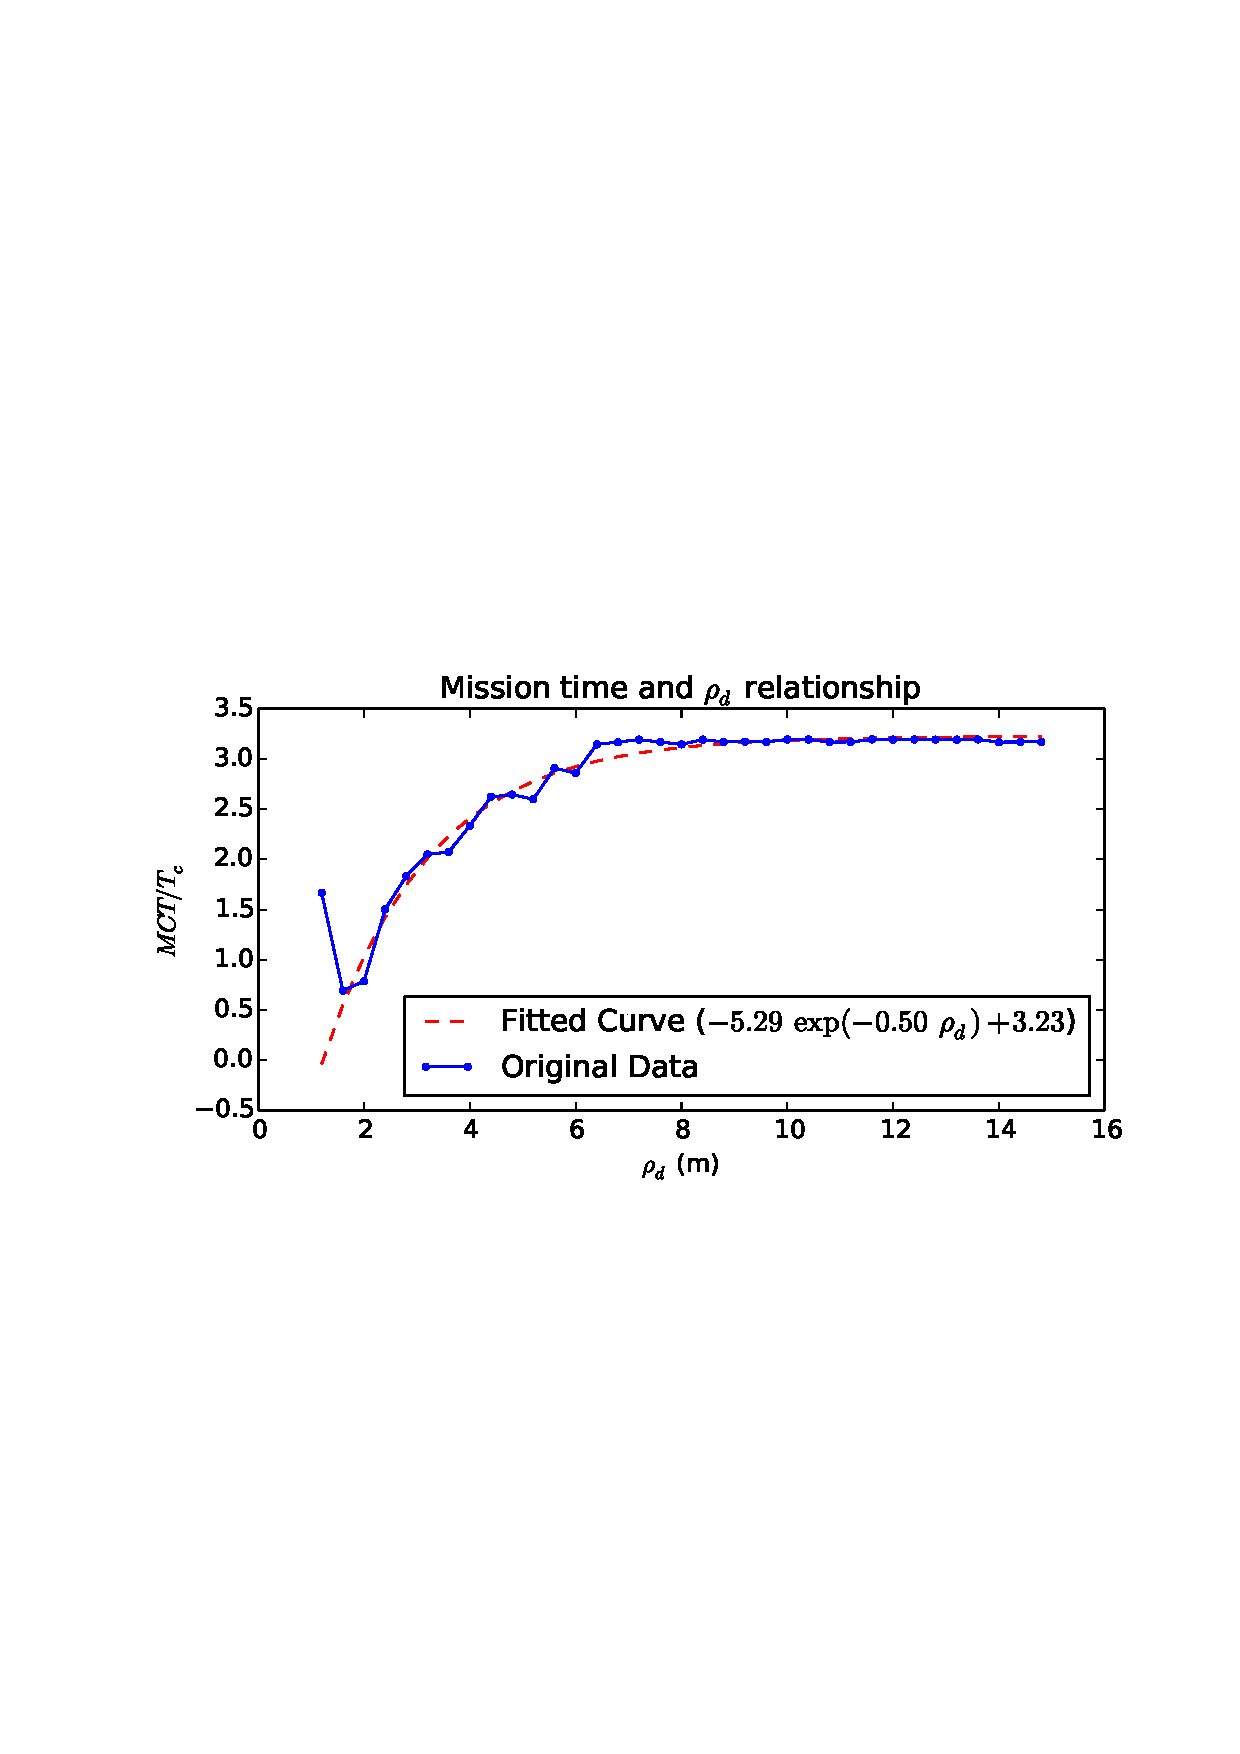
\includegraphics[width=\linewidth]{./images/drho/drho-rmp.pdf} % <-- use this
  %\rule{5cm}{5cm} % <-- this is just a black box substitute for graphics
  \caption{Increasing of detection radius and impact on a $MTC/T_c$ 
ratio\label{fig:drho}}
\label{fig:res}
\end{figure}

\subsection{Obstacle penetration $P$}

\ref{fig:pen}
TODO rescale images

\begin{figure}[!h]\centering
%  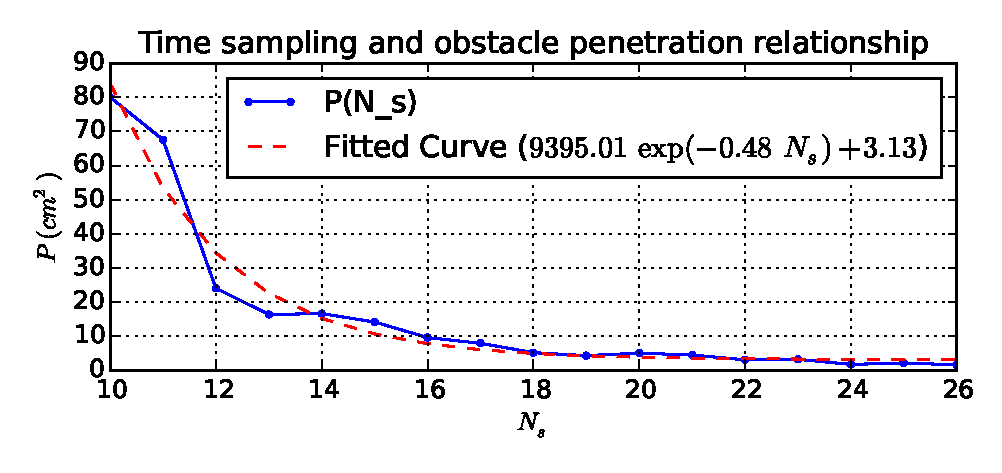
\includegraphics[width=\linewidth]{./images/penetration/pen-nsi.eps} %
  %\rule{5cm}{5cm} % <-- this is just a black box substitute for graphics
  \caption{Obstacle penetration decreasing as sampling increases\label{fig:pen}}
\label{fig:res}
\end{figure}




\subsection{Total execution time $T_{tot}$}



\subsection{Additional time for conflict handling$P$}


TODO Comparison with the other method;

TODO Before concluding do comparison with other approach and make sure to have 
multi-robot stuff

\section{Conclusions}



%\begin{nomenclature}
%\item[kg\,m^-3]{\varrho}{Liquid density}
%\item[Pa]{p}{Liquid pressure}
%\medskip
%\item{\mathit{Re}}{Reynold's number}

%\begin{acknowledgements}
%G.~Surname was supported by grant 1234567890.
%\end{acknowledgements}

TODO perspectives

Analise influence of dynamics of system, sensors, communication latency;

\bibliographystyle{actapoly}
\bibliography{biblio}

\end{document}
%kate: default-dictionary en;